\section{Revisione dei requisiti}
\begin{frame}
  \titlepage
\end{frame}

\begin{frame}

\begin{center} \usebeamerfont*{title} \usebeamercolor[fg]{title} \huge Studio di fattibilità \end{center}

\end{frame}

\section{Studio di fattibilità}
\begin{frame}
  \frametitle{Capitolato scelto - MaaS}
  \begin{columns}
    \begin{column}{0.4\textwidth}
      \par{\textbf{Aspetti positivi:}}
      \begin{itemize}
      \item Requisiti utente ben delineati;
      \item Disponibilità del proponente nella negoziazione dei requisiti.
      \item Uso di tecnologie innovative e richieste dal mercato.
      \end{itemize}
    \end{column}
    \begin{column}{0.4\textwidth}
      
\includegraphics[width=0.6\columnwidth]{maas.png}\\
      
\includegraphics[width=0.5\columnwidth]{mongodb.png}\\
      
\includegraphics[width=0.5\columnwidth]{node.png}\\
      
\includegraphics[width=0.4\columnwidth]{react.png}\\
      
\includegraphics[width=0.5\columnwidth]{angular.png}
    \end{column}
  \end{columns}
\end{frame}

\begin{frame}
  \frametitle{Capitolato scelto - MaaS}
  \par{\textbf{Aspetti negativi:}}
  \begin{itemize}
  \item Alcuni membri del gruppo non hanno competenze avanzate nell’ambito di sviluppo del presente progetto;
  \item Nella prima fase la mole di lavoro per la realizzazione del progetto appare notevole.
  \end{itemize}
\end{frame}

\begin{frame}
  \frametitle{Altri capitolati - ActorBase}
  \begin{columns}
    \begin{column}{0.4\textwidth}
      \par{\textbf{Aspetti positivi:}}
      \begin{itemize}
      \item Gli argomenti trattati sono interessanti per il gruppo;
      \item Opportunità di apprendere un linguaggio moderno e innovativo come \textit{Scala}.
      \end{itemize}
    \end{column}
    \begin{column}{0.4\textwidth}
      \par{\textbf{Aspetti negativi:}}
      \begin{itemize}
      \item Progetto interno all'università;
      \item Tempi di sviluppo troppo lunghi.
      \end{itemize}
    \end{column}
  \end{columns}
\end{frame}

\begin{frame}
  \frametitle{Altri capitolati - CLIPS}
  \begin{columns}
    \begin{column}{0.4\textwidth}
      \par{\textbf{Aspetti positivi:}}
      \begin{itemize}
      \item Area di studio interessante ed innovativa
      \end{itemize}
    \end{column}
    \begin{column}{0.4\textwidth}
      \par{\textbf{Aspetti negativi:}}
      \begin{itemize}
      \item Tempi molto lunghi per l'analisi dei requisiti (con rischio di ritardare la consegna);
      \item Descrizione degli obiettivi del progetto poco chiara.
      \end{itemize}
    \end{column}
  \end{columns}
  
\includegraphics[width=0.3\textwidth]{miriade.png}
\end{frame}

\begin{frame}
  \frametitle{Altri capitolati - UMAP}
  \begin{columns}
    \begin{column}{0.4\textwidth}
      \par{\textbf{Aspetti positivi:}}
      \begin{itemize}
      \item Utilità del prodotto richiesto;
      \item Uso di tecnologie innovative e richieste dal mercato.
      \end{itemize}
    \end{column}
    \begin{column}{0.4\textwidth}
      \par{\textbf{Aspetti negativi:}}
      \begin{itemize}
      \item Ideazione impegnativa dell'algoritmo predittivo.
      \end{itemize}
    \end{column}
  \end{columns}
  \centering
  
\includegraphics[width=0.3\textwidth]{umap.png}
\end{frame}

\begin{frame}
  \frametitle{Altri capitolati - Quizzipedia}
  \begin{columns}
    \begin{column}{0.4\textwidth}
      \par{\textbf{Aspetti positivi:}}
      \begin{itemize}
      \item Requisiti minimi ben delineati;
      \item Libertà nello sviluppo di funzionalità opzionali;
      \item Uso di tecnologie innovative e richieste dal mercato.
      \end{itemize}
    \end{column}
    \begin{column}{0.4\textwidth}
      \par{\textbf{Aspetti negativi:}}
      \begin{itemize}
      \item Scarsamente sfidante nelle richieste e nello scopo
      \end{itemize}
    \end{column}
  \end{columns}
  \centering
  
\includegraphics[width=0.3\textwidth]{quizzpedia.png}
\end{frame}

\begin{frame}
  \frametitle{Altri capitolati - SiVoDiM}
  \begin{columns}
    \begin{column}{0.4\textwidth}
      \par{\textbf{Aspetti positivi:}}
      \begin{itemize}
      \item Prevista facilità nella realizzazione;
      \item Chiarezza delle richieste.
      \end{itemize}
    \end{column}
    \begin{column}{0.4\textwidth}
      \par{\textbf{Aspetti negativi:}}
      \begin{itemize}
      \item Non è considerato dal gruppo un banco di prova per l'apprendimento di nuove tecnologie.
      \end{itemize}
    \end{column}
  \end{columns}
\centering

\includegraphics[width=0.3\textwidth]{mivoq.png}
\end{frame}

\begin{frame}

\begin{center} \usebeamerfont*{title} \usebeamercolor[fg]{title} \huge Norme di progetto \end{center}

\end{frame}

\section{Norme di progetto}
\begin{frame}
  \frametitle{Processi primari}
  Il documento è stato suddiviso per processi.
  \begin{itemize}
  \item Processi primari
    \begin{itemize}
    \item Processo di sviluppo\\
      Vengono stabilite modalità, norme e strumenti per regolare l'attività di analisti, progettisti e programmatori.
      \begin{itemize}
      \item Attività di analisi dei requisiti\\
        
\includegraphics[width=0.2\textwidth]{astah.png}
        
\includegraphics[width=0.1\textwidth]{uml.jpg}
      \item Attività di progettazione\\
        
\includegraphics[width=0.1\textwidth]{uml.jpg}
      \item Attività di codifica\\
        
\includegraphics[width=0.1\textwidth]{emacs.png}
        
\includegraphics[width=0.2\textwidth]{webstorm.png}
      \end{itemize}
    \end{itemize}
  \end{itemize}
\end{frame}

\begin{frame}
  \frametitle{Processi di supporto}
  \begin{itemize}
  \item Processi di supporto
    \begin{itemize}
    \item Processo di documentazione\\
      Viene stabilito come dovrà essere gestita la documentazione, definendo delle regole da seguire nella stesura dei documenti.\\
      
\includegraphics[width=0.15\textwidth]{latex.png}
      
\includegraphics[width=0.1\textwidth]{emacs.png}
    \item Processo di verifica\\ Ha l'obiettivo di verificare che ogni componente prodotta durante il ciclo di vita del software sia conforme agli standard decisi dal Team (di qualità, relativi alle Norme di Progetto\dots).\\
      
\includegraphics[width=0.2\textwidth]{github.png}
    \end{itemize}
  \end{itemize}
\end{frame}

\begin{frame}
  \frametitle{Processi organizzativi}
  \begin{itemize}
  \item Processi organizzativi
    \begin{itemize}
    \item Processo di pianificazione\\
      Viene stabilito come suddividere il lavoro tra i componenti del Team, come effettuare la rotazione dei ruoli e come gestire le revisioni di progetto.\\
      
\includegraphics[width=0.2\textwidth]{gantt.png}
      
\includegraphics[width=0.2\textwidth]{teamwork.png}
    \end{itemize}
  \end{itemize}
\end{frame}

\begin{frame}

\begin{center} \usebeamerfont*{title} \usebeamercolor[fg]{title} \huge Piano di qualifica \end{center}

\end{frame}

\section{Piano di qualifica}
\begin{frame}
  \frametitle{Standard di qualità}
  Il gruppo, con lo scopo di assicurare la qualità dei processi usati e del prodotto sviluppato, ha deciso di seguire gli standard:
	\begin{itemize}
  	\item \textbf{Standard ISO/IEC 15504}
  	\item \textbf{Standard ISO/IEC 9126}
	\end{itemize}
\end{frame}

\begin{frame}
  \frametitle{Vantaggi}
  \begin{columns}
    \begin{column}{0.4\textwidth}
Vantaggi nel controllo della \textbf{qualità dei processi}:
	\begin{itemize}
  	\item Ottimizzazione dell’uso di risorse;
  	\item Contenimento dei costi;
  	\item Migliore stima dei rischi e degli impegni.
	\end{itemize}
	\centering
	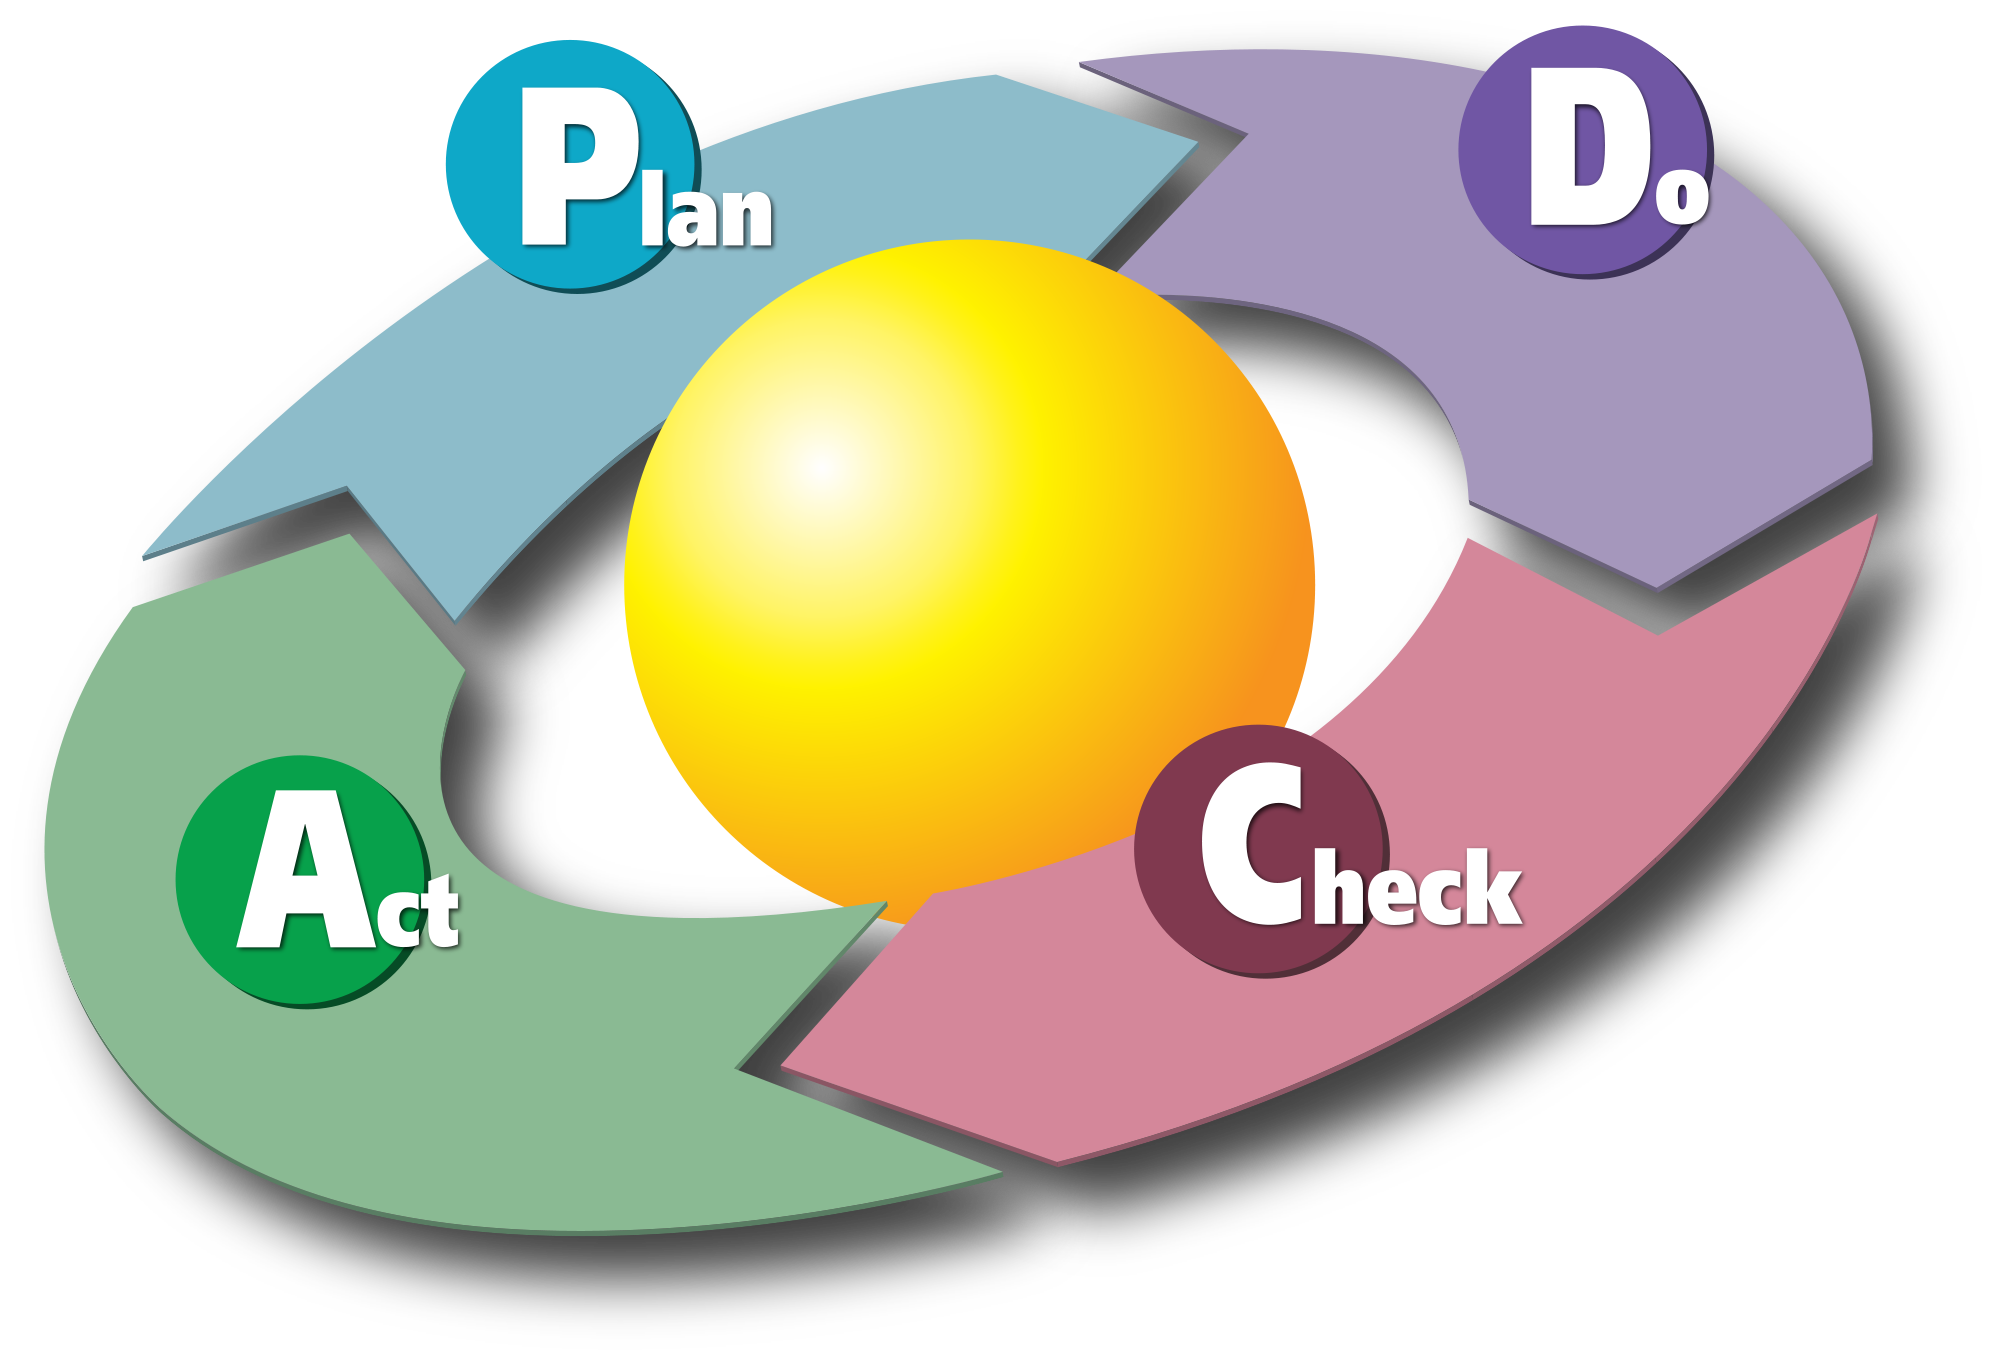
\includegraphics[width=0.6\textwidth]{pdca.png}
	\end{column}
	\begin{column}{0.4\textwidth}
	Vantaggi nel controllo della \textbf{qualità di prodotto}:
	\begin{itemize}
  	\item Disponibilità di un modello di qualità da seguire;
  	\item Disponibilità di metriche per la qualità esterna, interna e in uso.
	\end{itemize}
	\end{column}
   \end{columns}
\end{frame}

\begin{frame}
  \frametitle{Metriche}
  Al termine della stesura e della verifica dei documenti in ingresso alla revisione dei requisiti, ne abbiamo calcolato l'indice di leggibilità utilizzando l'indice di Gulpease.
\end{frame}

